\chapter[Chapter 3-TBD]{Chapter 3 Title}
\label{sec:chapter3}
\setcounter{secnumdepth}{3}
%
%% Brief summary of chapter
%
\minitoc
%

%%%%%%%%%% Chapter 3 - Section 1
	\section{Chapter 3 - Section 1}
\label{sec:chapter_3_sec_1}

\subsection{Chpt 3 - Sec 1 - Subsection 1 - TBD}

\subsection{Chpt 3 - Sec 1 - Subsection 2 - TBD}



%%%%%%%%%% Chapter 3 - Section 2
	\section{Chapter 3 - Section 2}
\label{sec:chapter_3_sec_2}


\subsection{Example reference and citations}


Here is a reference to table \ref{table:template}.

Here is a citation to \cite{cappanera2018momentum}.

\subsection{Example Table}


\begin{table}[ht]
    \centering
    \begin{tabular}{|l|l|l||l|l||l|l|}
    \hline
         $\tau$ & \multicolumn{2}{|c||}{Velocity}   & \multicolumn{2}{c||}{Pressure} & \multicolumn{2}{c|}{Density}  \\ \hline
         & $L^2$ error & Rate & $L^2$ error & Rate & $L^2$ error & Rate \\ \hline
        0.05   	& 1.63E-3  & - 	&  8.61E-2 &- & 1.96E-2 & - \\ \hline
        0.025   & 4.32E-4 & 1.91 & 3.01E-2 & 1.51 & 1.22E-2 & 0.69 \\ \hline
        0.0125  & 1.60E-4 & 1.43 & 8.73E-3 & 1.79 & 6.45E-3 & 0.92 \\ \hline
        0.00625 & 6.58E-5 & 1.28 & 2.39E-3 & 1.87 & 3.02E-3 & 1.09 \\ \hline
        0.003125& 3.37E-5 & 0.96 & 9.21E-4 & 1.38 & 1.57E-3 & 0.94  \\ \hline
    \end{tabular}
\caption[Template table-description for list of tables.]{Results of convergence test for smooth density with $(\rho_1,\rho_2)=(1,3)$ and $\tau=h/10$.}
\label{table:template}
\end{table}


\subsection{Example Figure}

\begin{figure}[H]
     \centering         
     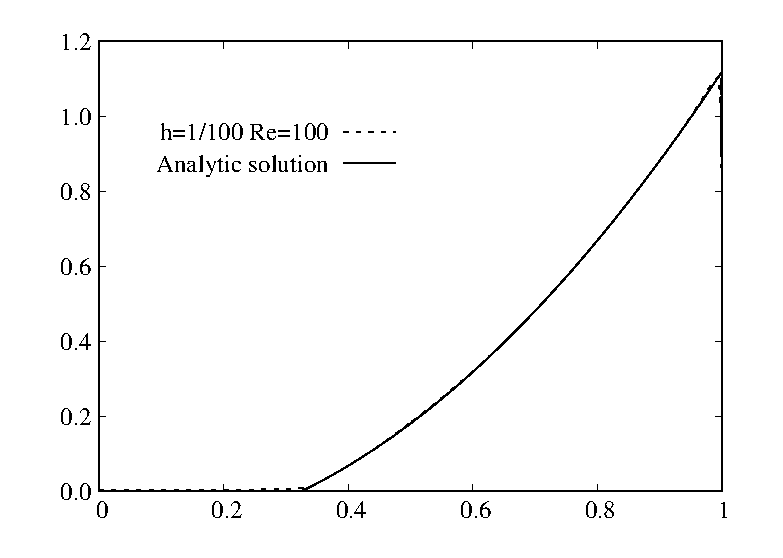
\includegraphics[width=0.6\textwidth]{Newton_profile_dry_A} 
     \caption[Template figure-description for list of figures.]{Description figure.}
     \label{fig:template-fig}
\end{figure}

\subsection{Example SubFigure}


\begin{figure}[H]
     \centering
     \begin{subfigure}[H]{0.31\textwidth} % Re = 100, dry
         \centering
         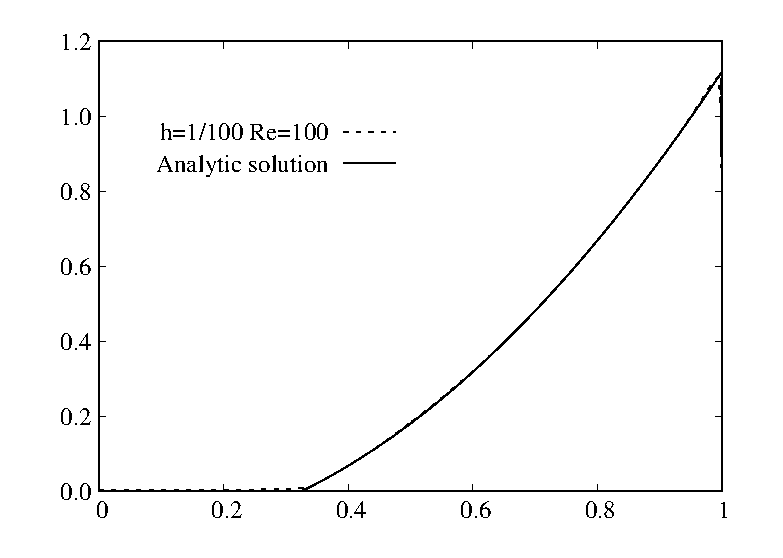
\includegraphics[width=\textwidth]{Newton_profile_dry_A} 
         \caption{$R_e=100.$}
         \label{fig:template-subfig-1}
     \end{subfigure}
     \hfill
     \begin{subfigure}[H]{0.31\textwidth} % Re = 500, dry
         \centering
         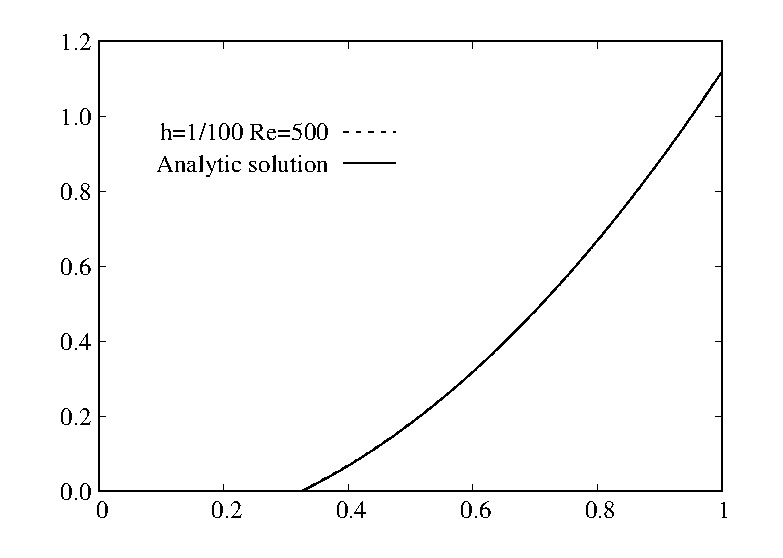
\includegraphics[width=\textwidth]{Newton_profile_dry_C}
         \caption{$R_e=500.$}
         \label{fig:dry_Re_500}
         \label{fig:template-subfig-2}
     \end{subfigure}
     \hfill
     \begin{subfigure}[H]{0.31\textwidth} % Re = 1000, dry
         \centering
         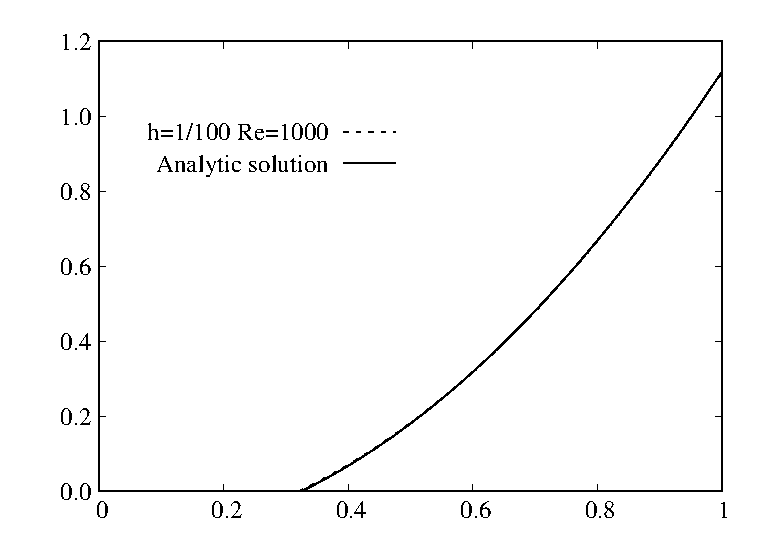
\includegraphics[width=\textwidth]{Newton_profile_dry_B}
         \caption{$R_e=1000$}
         \label{fig:template-subfig-3}
     \end{subfigure}
        \caption[Template subfigure-description for list of figures.]{Contour plots of fluid surface, dry case, $F_r=2.5,\rho = (0.001,1)$.}
        \label{fig:template-subfig}
\end{figure}



